% !TEX root = ../main.tex
\section{Appendix}

\begin{figure}[H]
\centering
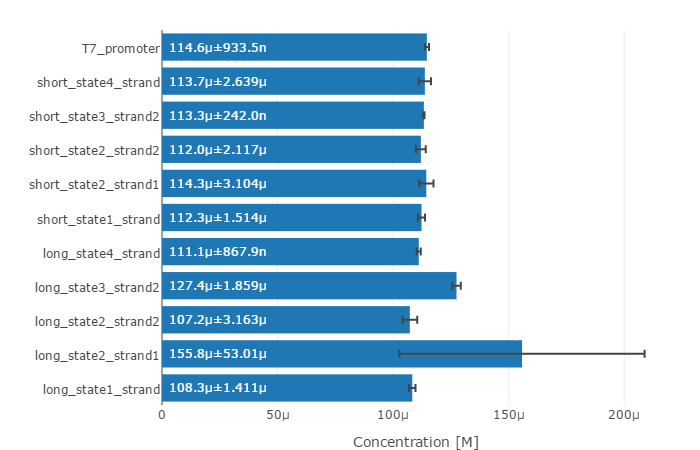
\includegraphics[width=\columnwidth]{images/oligo_concentrations.png}
\caption{Concentrations of the dissolved DNA oligos ordered from IDT.}
\label{oligo_concentrations}
\end{figure}

\begin{figure}[H]
\centering
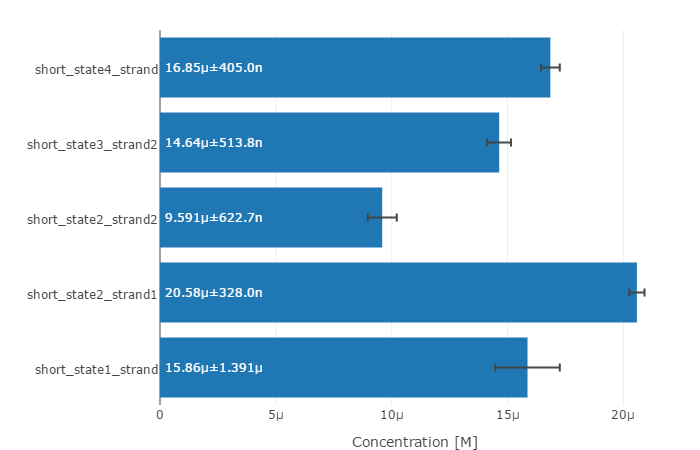
\includegraphics[width=\columnwidth]{images/translator_transcription_concentration.png}
\caption{Concentrations of the short translator RNA sequences.}
\label{translator_transcription_concentration}
\end{figure}


\begin{figure}
\begin{subfigure}{.32\columnwidth}
  \centering
  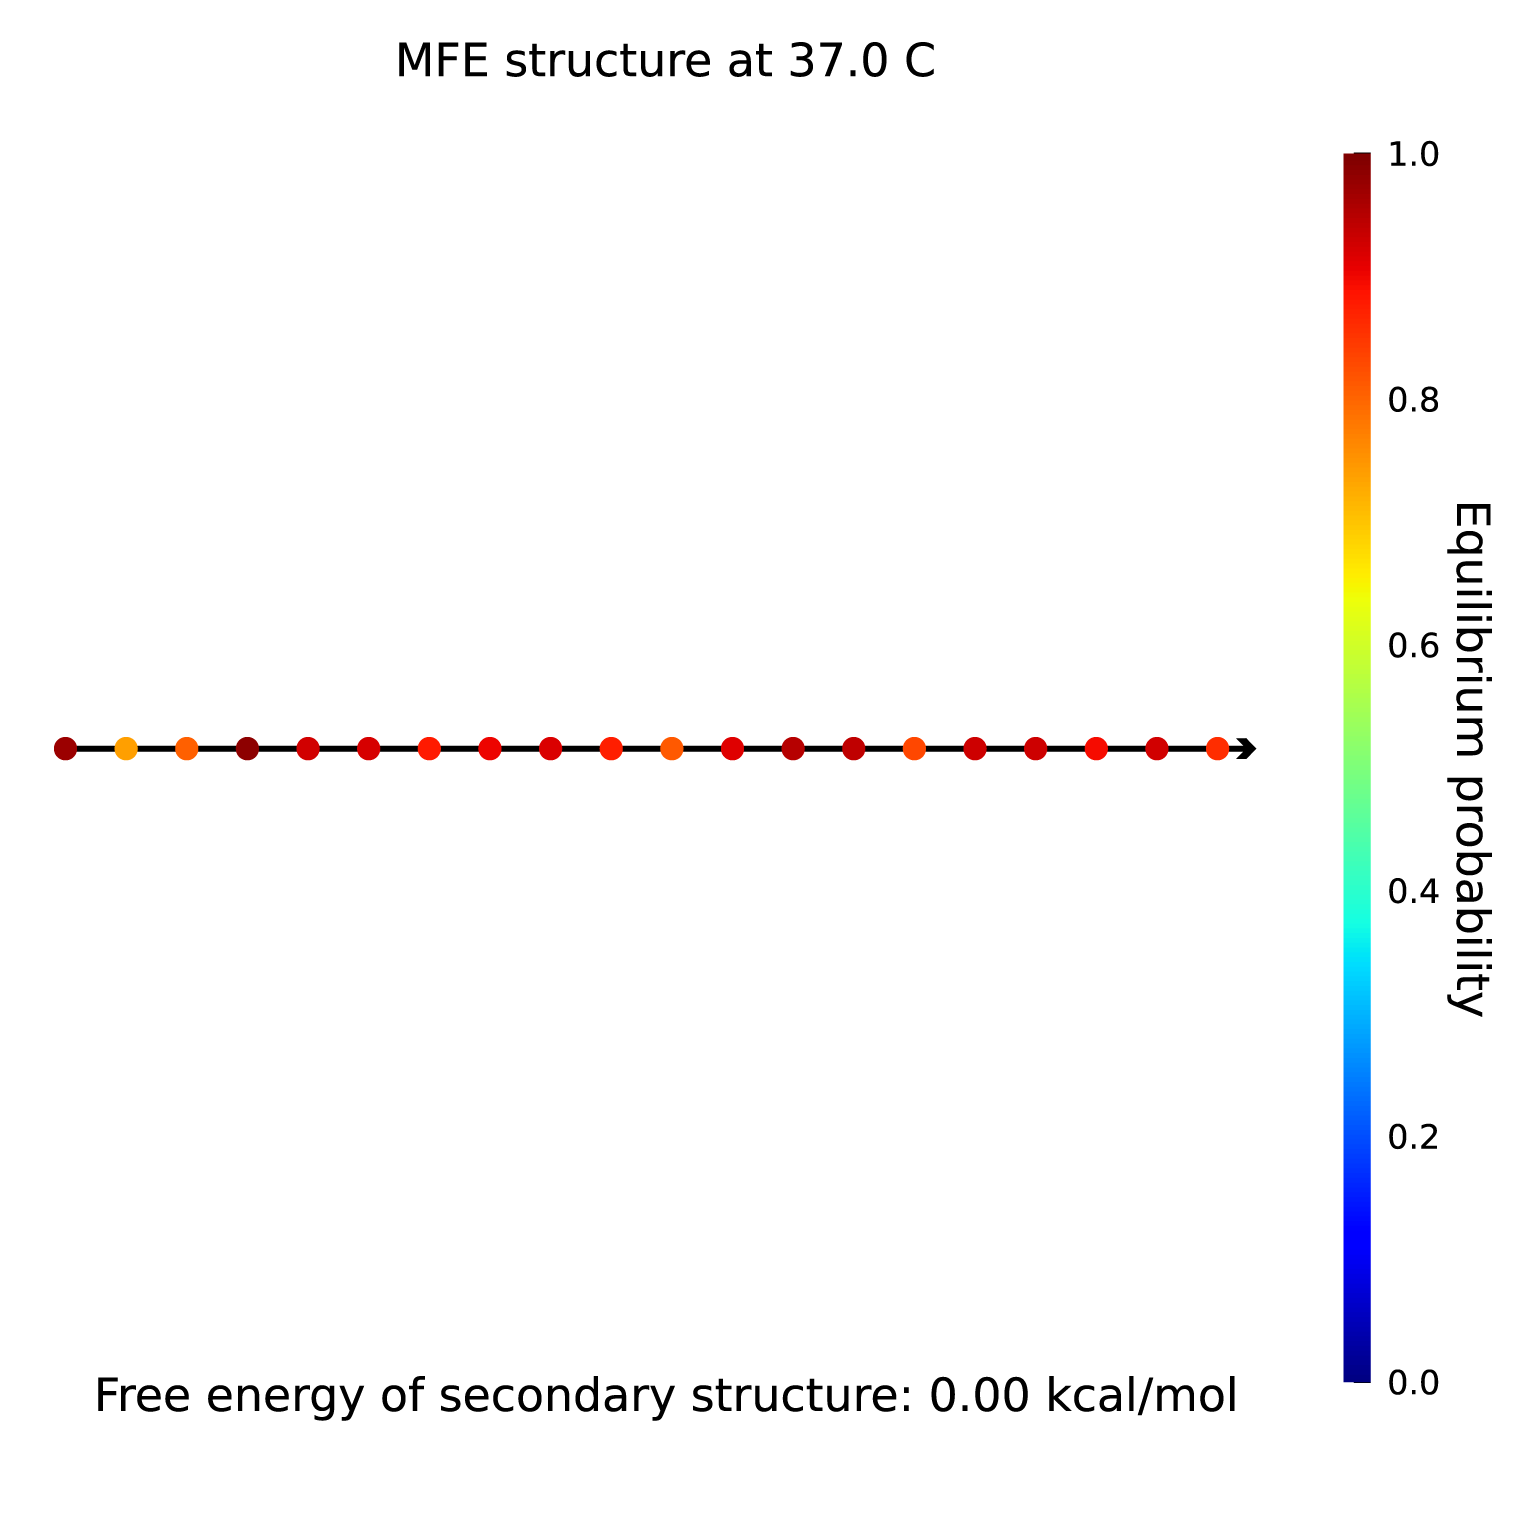
\includegraphics[width=\linewidth]{images/0_analysis.png}
  \caption{T7 promoter}
\end{subfigure}%
\begin{subfigure}{.32\columnwidth}
  \centering
  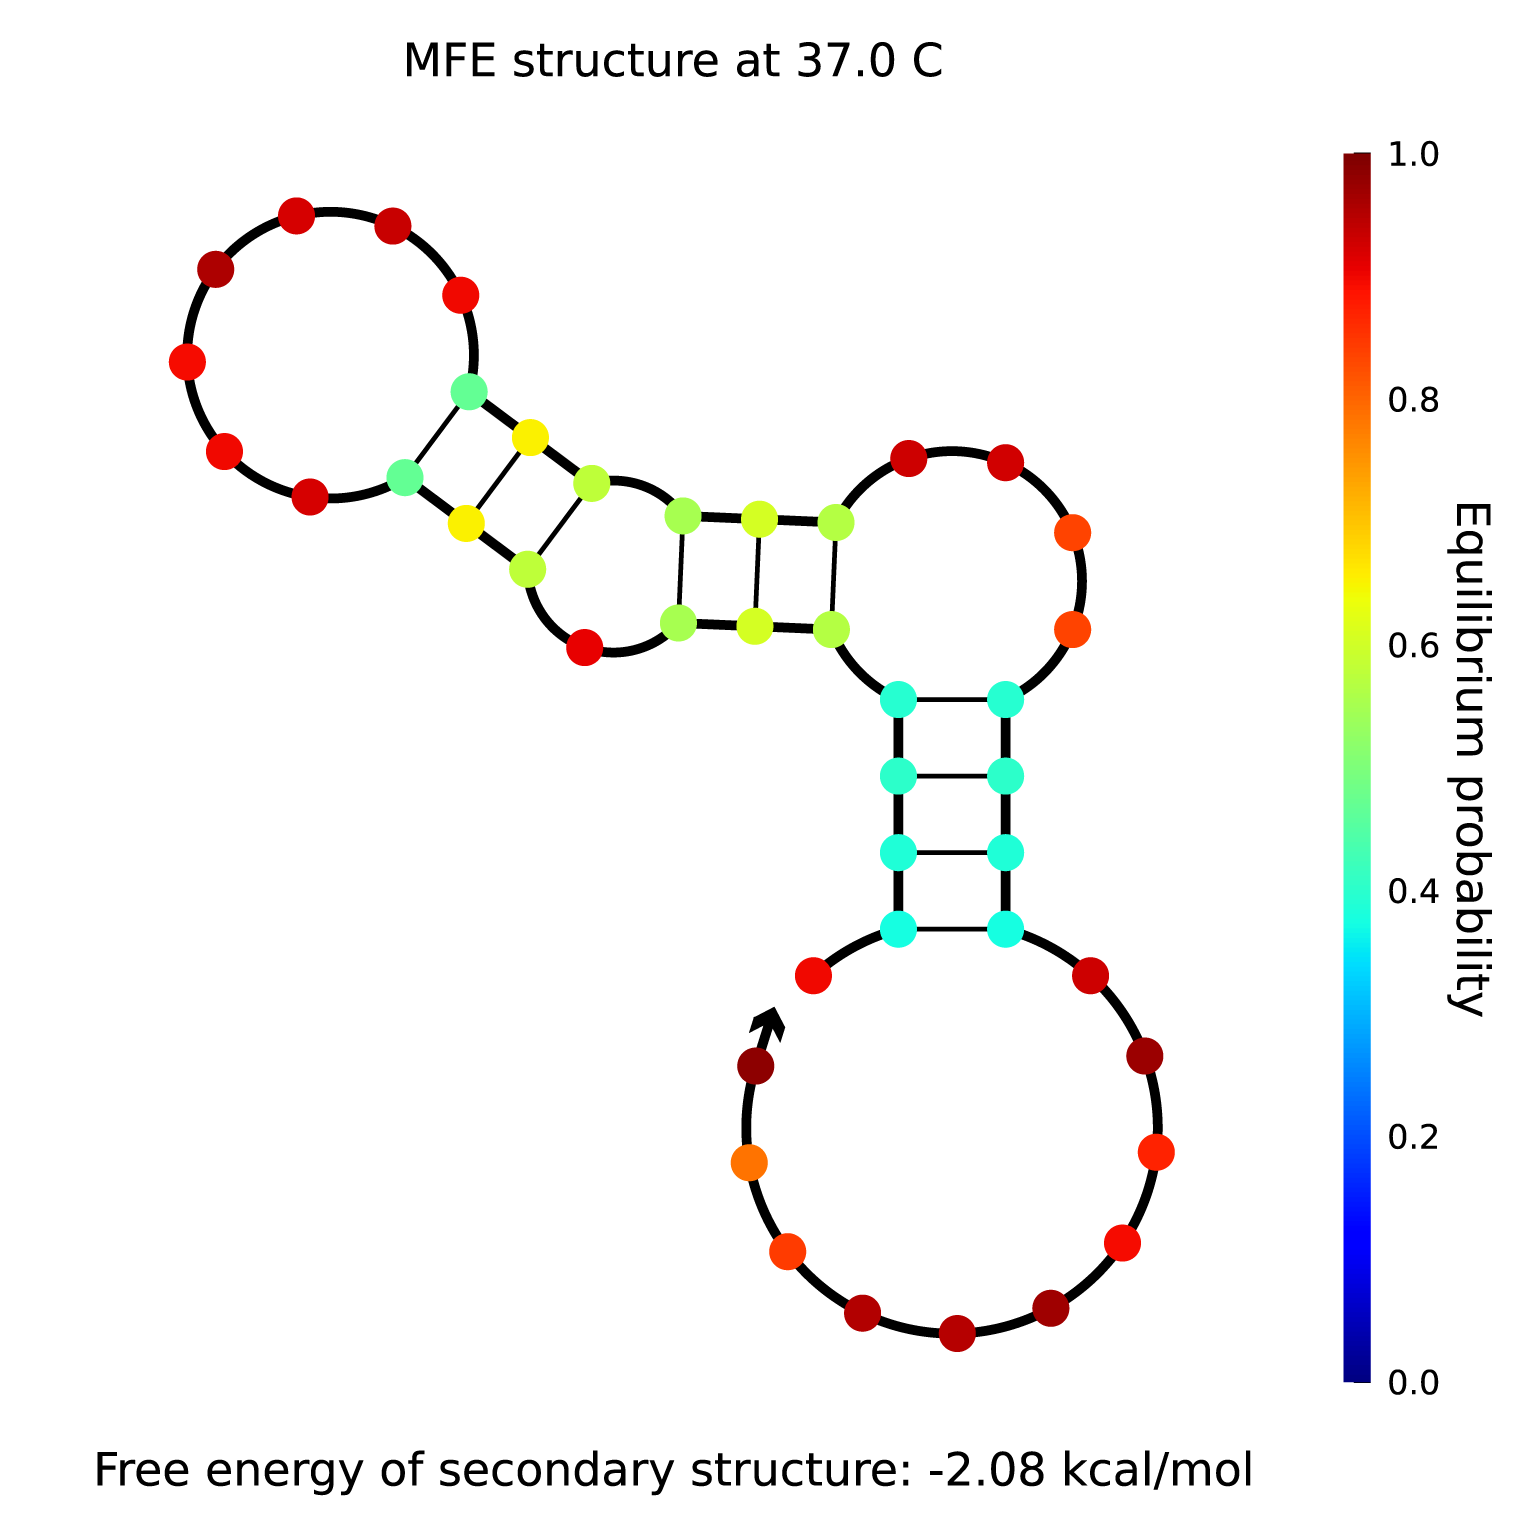
\includegraphics[width=\linewidth]{images/1_analysis.png}
  \caption{Short 1}
\end{subfigure}
\begin{subfigure}{.32\columnwidth}
  \centering
  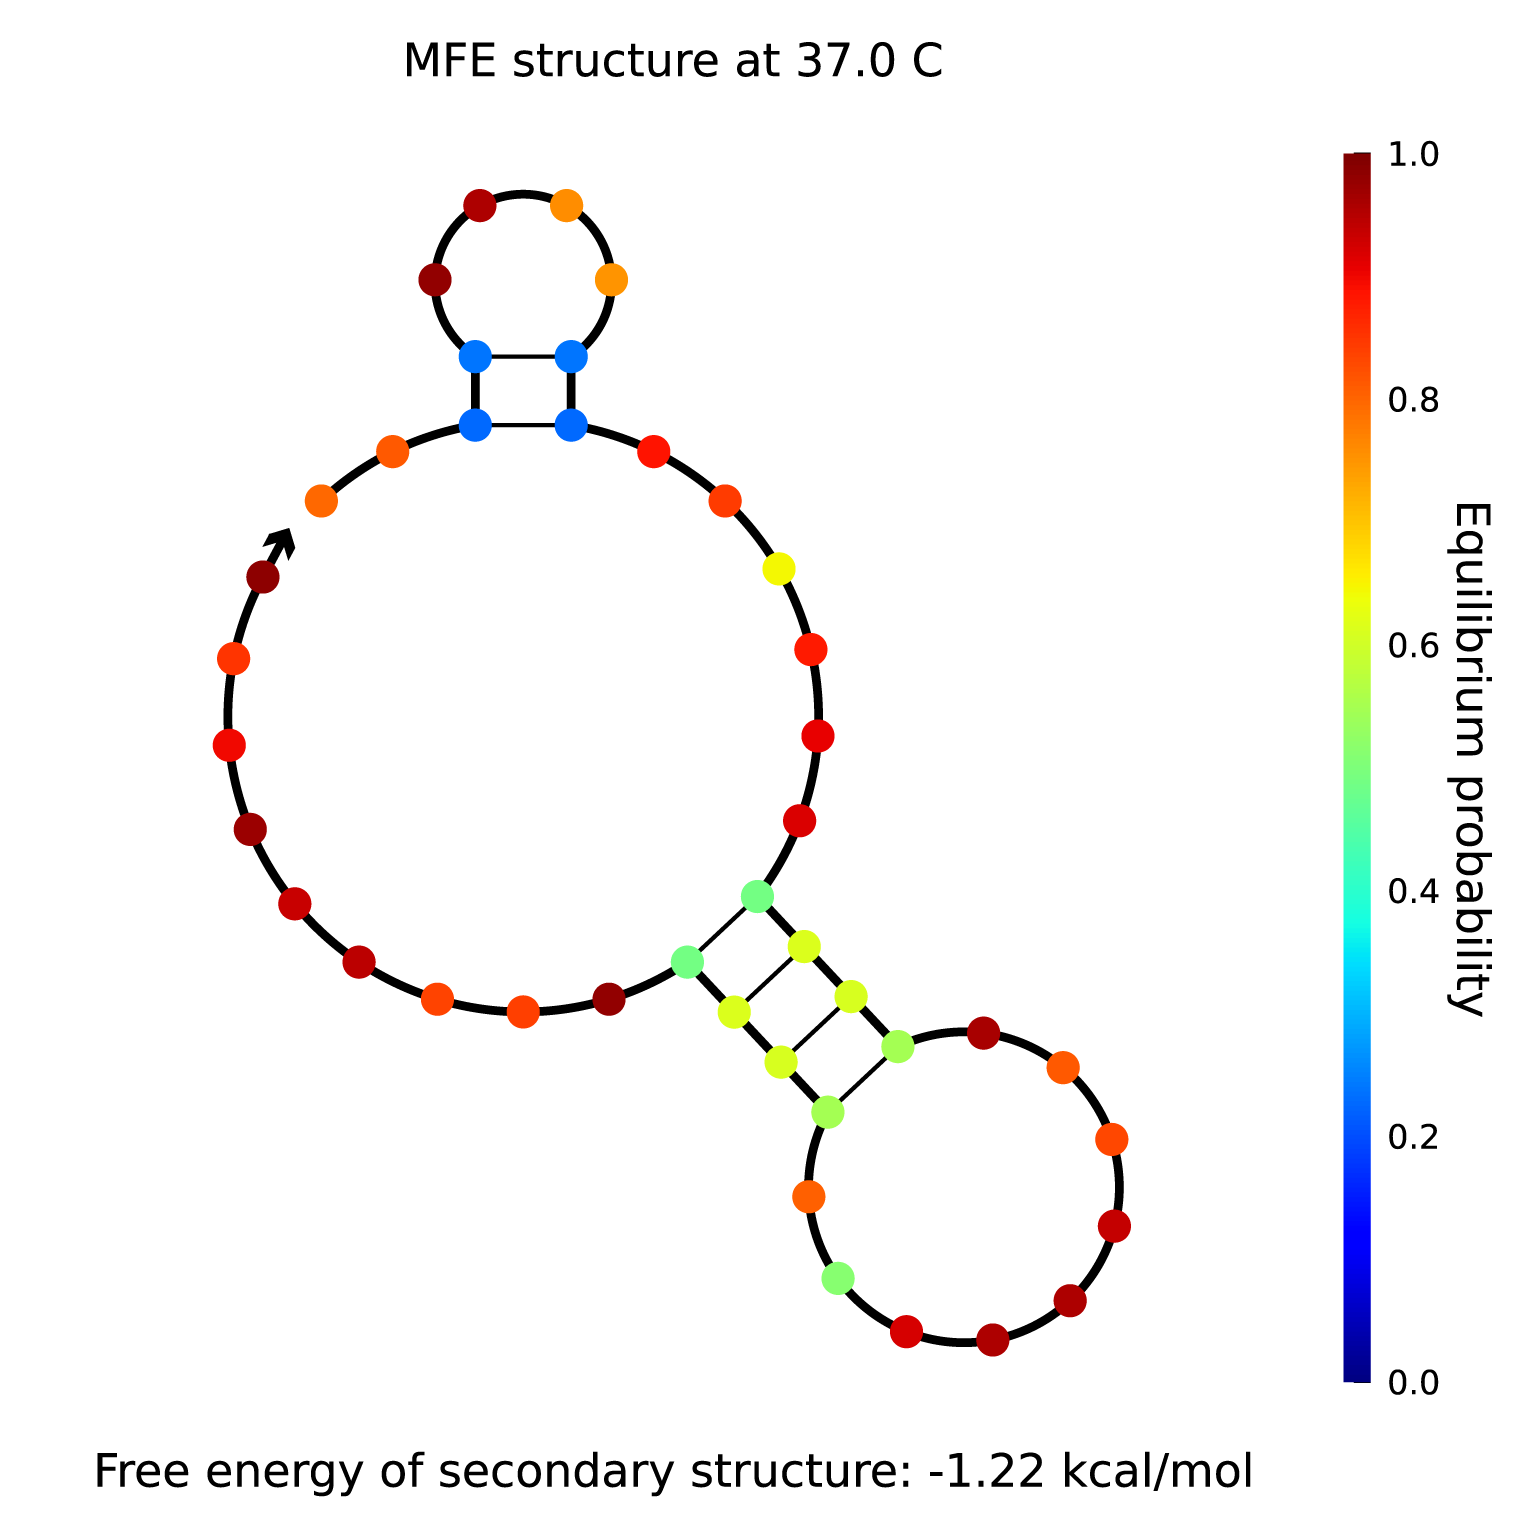
\includegraphics[width=\linewidth]{images/2_analysis.png}
  \caption{Short 2}
\end{subfigure}
\begin{subfigure}{.32\columnwidth}
  \centering
  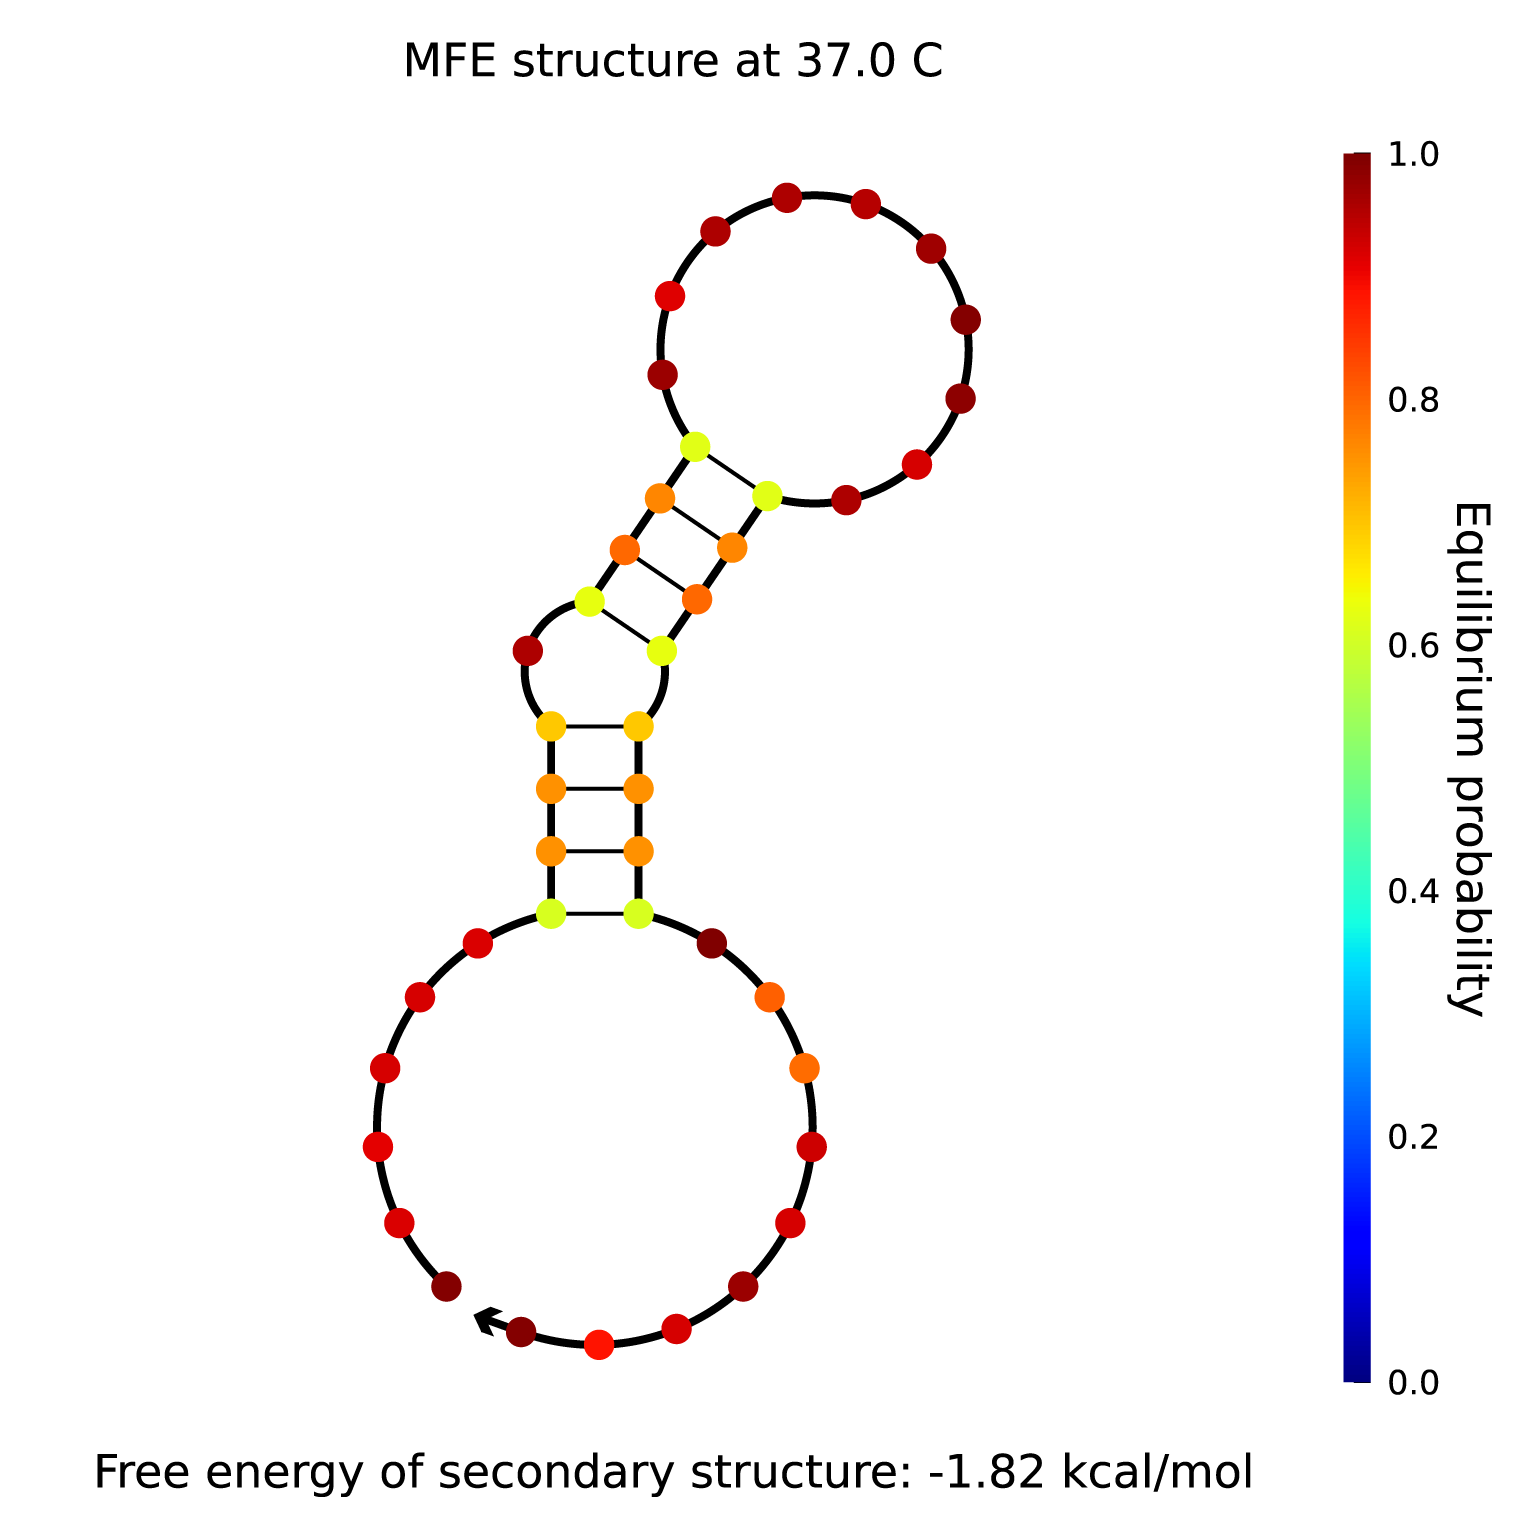
\includegraphics[width=\linewidth]{images/3_analysis.png}
  \caption{Short 3}
\end{subfigure}
\begin{subfigure}{.32\columnwidth}
  \centering
  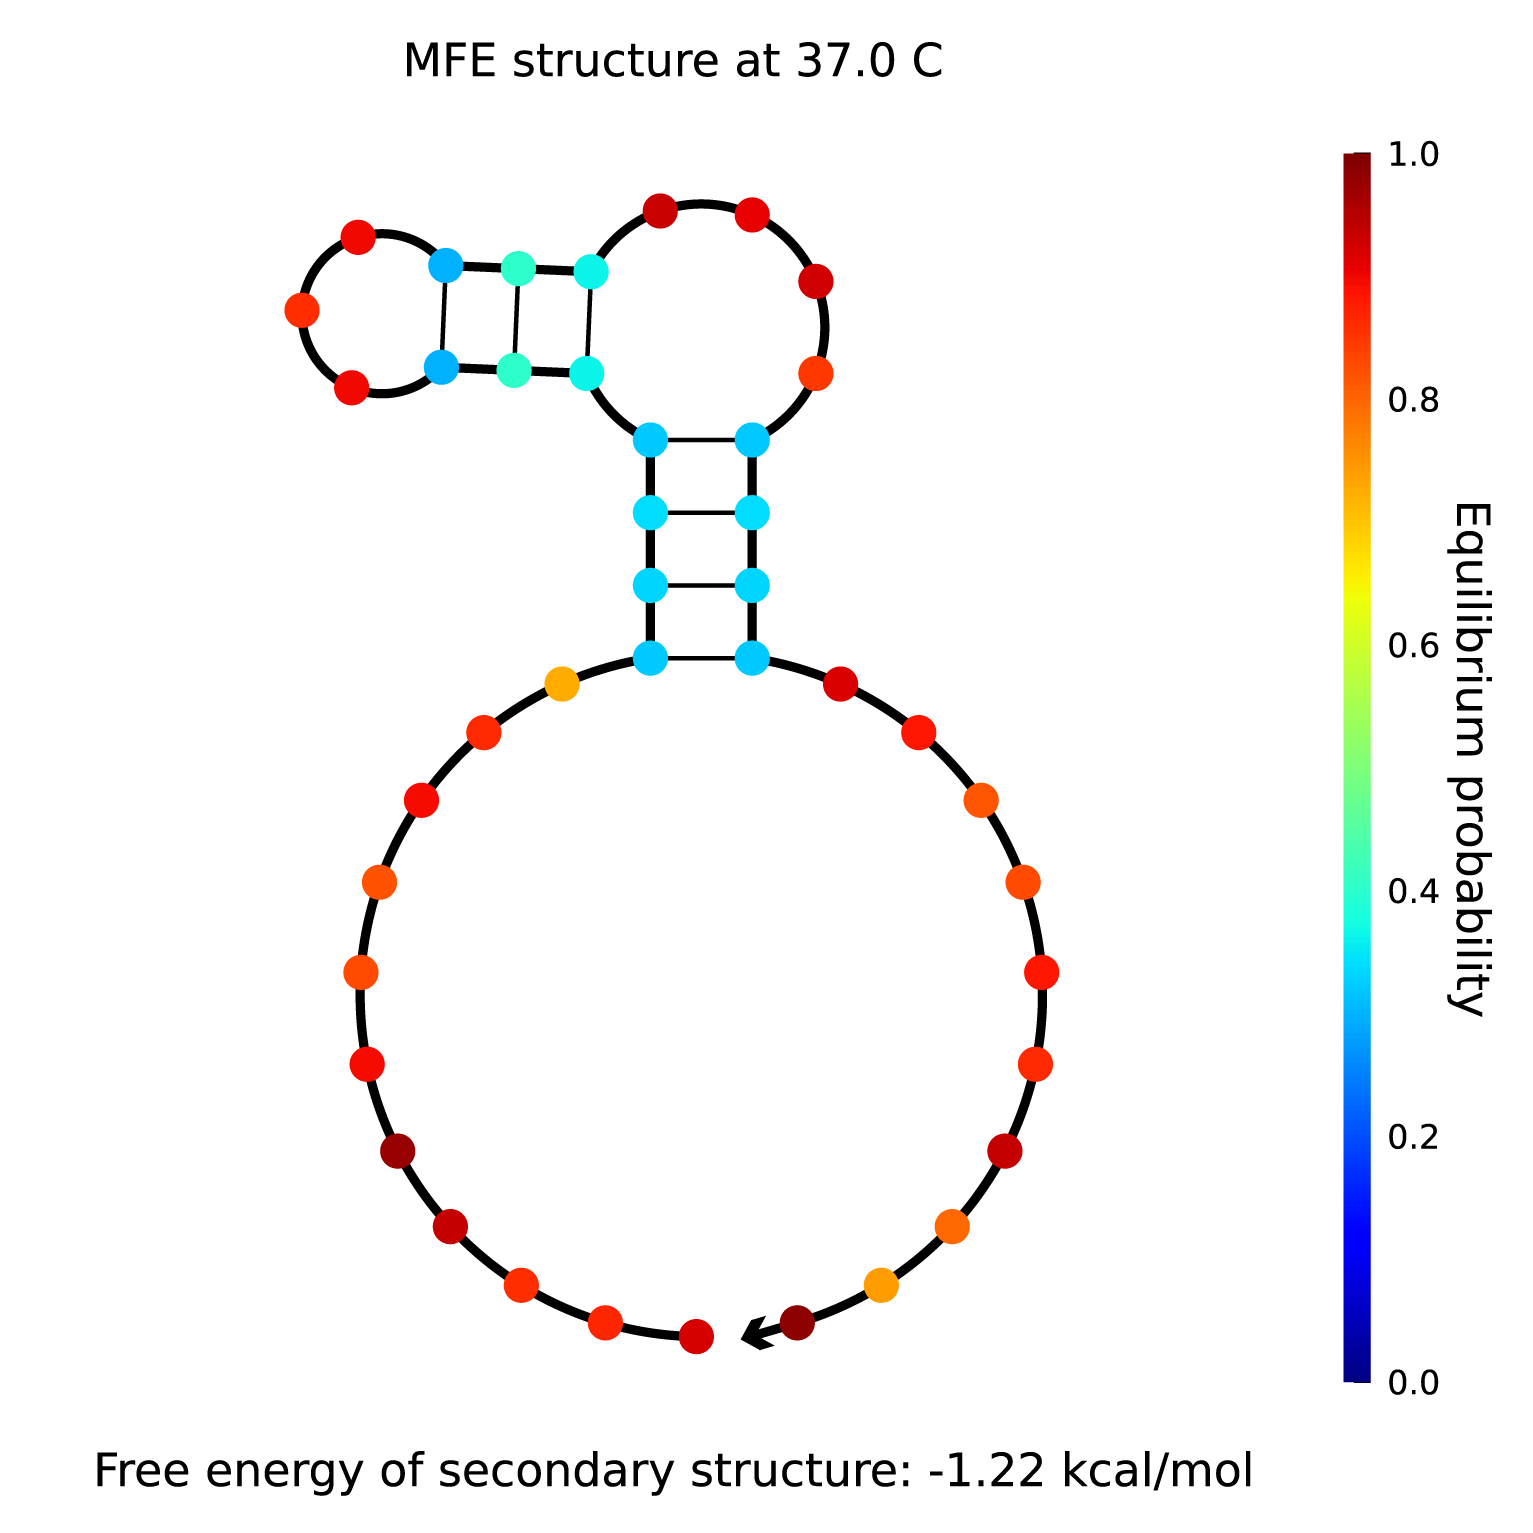
\includegraphics[width=\linewidth]{images/4_analysis.png}
  \caption{Short 4}
\end{subfigure}
\begin{subfigure}{.32\columnwidth}
  \centering
  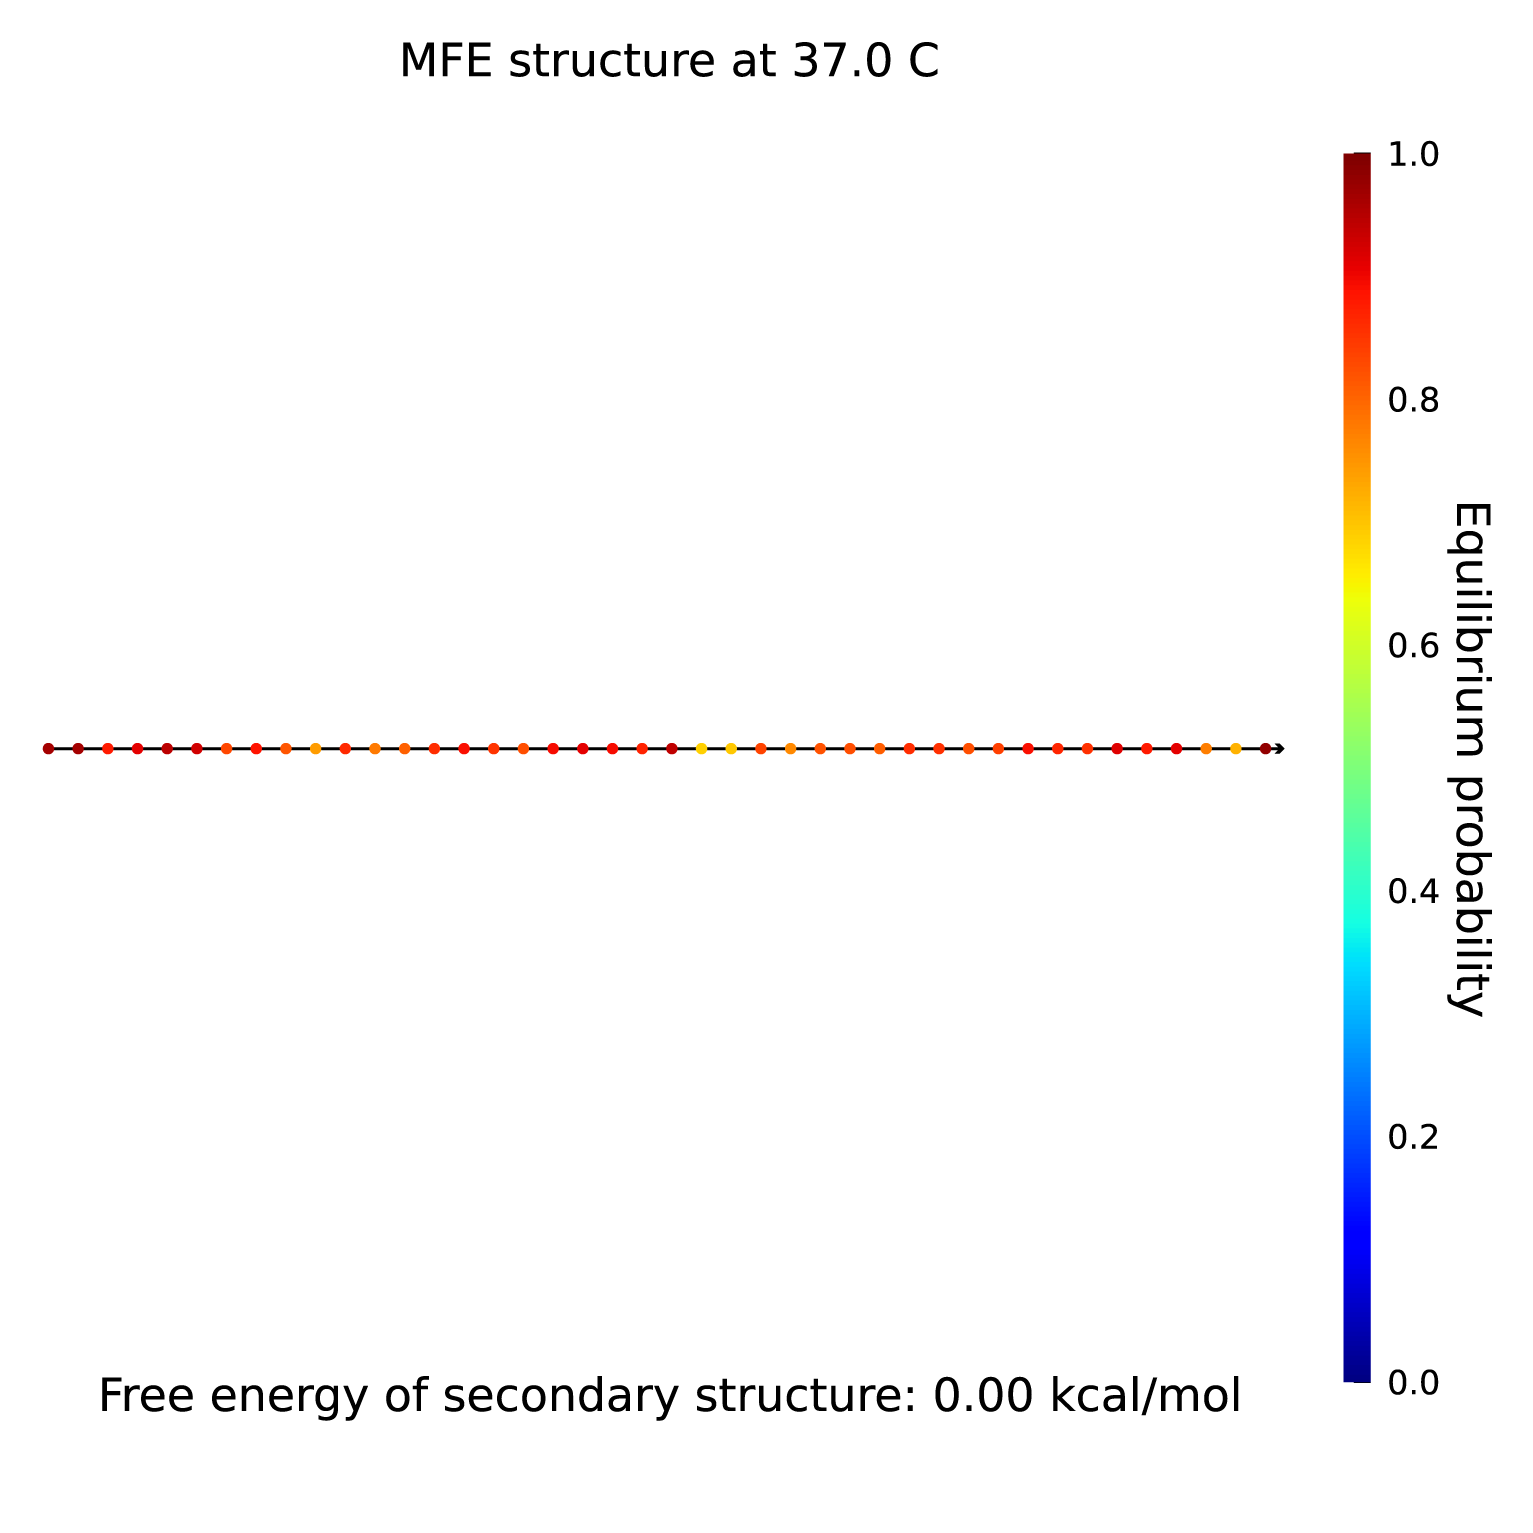
\includegraphics[width=\linewidth]{images/5_analysis.png}
  \caption{Short 5}
\end{subfigure}
\caption{Secondary structures of the DNA sequences for the short translator and the T7 promoter sequence.}
\label{short_secondary_structures}
\end{figure}

\begin{figure}
\begin{subfigure}{.32\columnwidth}
  \centering
  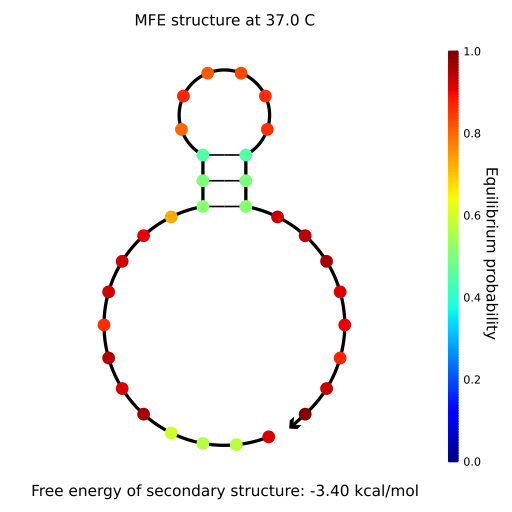
\includegraphics[width=\linewidth]{images/long_rna_secondarystructure_6.png}
  \caption{Long 6}
\end{subfigure}%
\begin{subfigure}{.32\columnwidth}
  \centering
  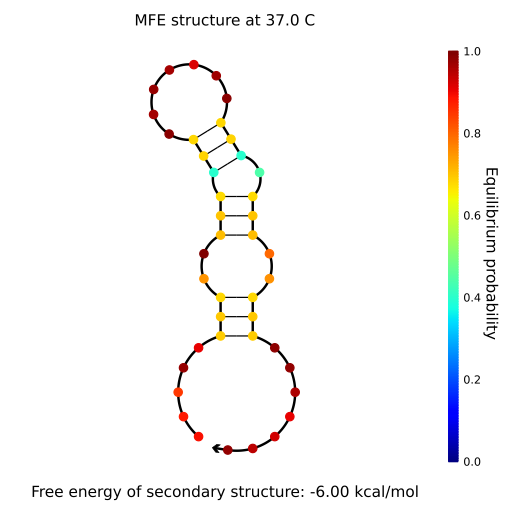
\includegraphics[width=\linewidth]{images/long_rna_secondarystructure_7.png}
  \caption{Long 7}
\end{subfigure}
\begin{subfigure}{.32\columnwidth}
  \centering
  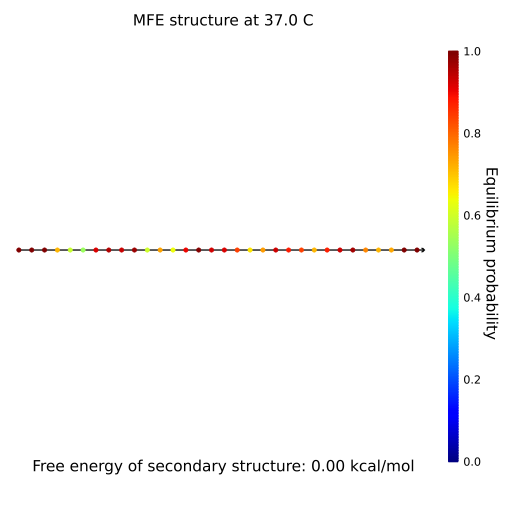
\includegraphics[width=\linewidth]{images/long_rna_secondarystructure_8.png}
  \caption{Long 8}
\end{subfigure}
\begin{subfigure}{.32\columnwidth}
  \centering
  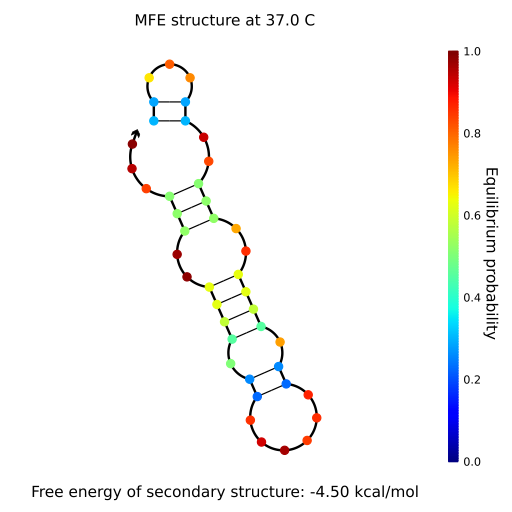
\includegraphics[width=\linewidth]{images/long_rna_secondarystructure_9.png}
  \caption{Long 9}
\end{subfigure}
\begin{subfigure}{.32\columnwidth}
  \centering
  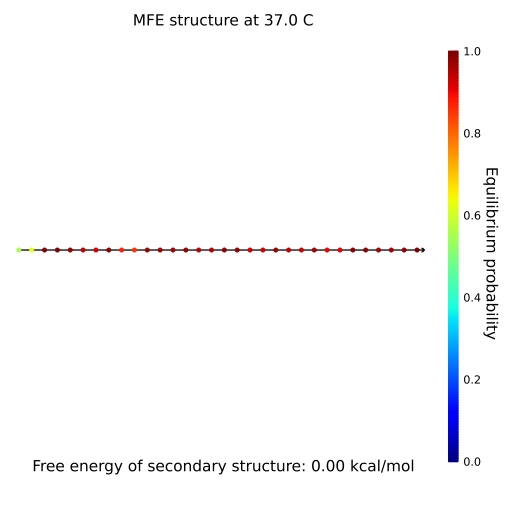
\includegraphics[width=\linewidth]{images/long_rna_secondarystructure_10.png}
  \caption{Long 10}
\end{subfigure}
\caption{Secondary structures of the RNA sequences for the long translator.}
\label{long_secondary_structures}
\end{figure}

\begin{table}
\centering
\begin{tabular}{ll}
  \hline
\textbf{}           & \textbf{Concentration} \\
\hline
Tris-HCl pH 8.0     & 10 nM                  \\
EDTA                & 1 mM                   \\
Nuclease-free water &               \\
\hline
\end{tabular}
\caption{Contents of 1X TE buffer.}
\label{te_buffer}
\end{table}

\begin{table}
\centering
\begin{tabular}{ll}
  \hline
\textbf{}           & \textbf{Concentration} \\
\hline
Tris pH 8.0     & 10 nM                  \\
NaCl                & 50 mM                   \\
EDTA                & 1 mM                   \\
Nuclease-free water &               \\
\hline
\end{tabular}
\caption{Contents of 1X annealing buffer.}
\label{annealing_buffer}
\end{table}

\begin{table}
\centering
\begin{tabular}{ll}
  \hline
\textbf{}           & \textbf{Concentration} \\
\hline
Xylene cyanol     & 0.04\%                 \\
Bromophenol blue                & 0.04\%                   \\
Glycerol                & 20\%                   \\
Nuclease-free water &               \\
\hline
\end{tabular}
\caption{Contents of native loading buffer.}
\label{native_buffer}
\end{table}

\begin{table}
\centering
\begin{tabular}{ll}
  \hline
\textbf{}           & \textbf{Concentration} \\
\hline
Xylene cyanol     & 0.04\%                 \\
Bromophenol blue                & 0.04\%                   \\
Glycerol                & 20\%                   \\
Urea & 5.4 M              \\
\hline
\end{tabular}
\caption{Contents of denaturing loading buffer.}
\label{denaturing_buffer}
\end{table}

\begin{lstlisting}[float,floatplacement=h,caption=Nupack code for the short translator, label=codeshort]
structure state1 = ......................
structure state2 = ............((((((((((+............))))))))))
structure state3 = .............((((((((((+............))))))))))
structure state4 = .......................

domain a = N10
domain b = N10
domain c = CUCCUUGAGG
domain d = CUAGACUGAAG
domain e = GG

state1.seq = e a b
state2.seq = e c a e b* a*
state3.seq = e d c e a* c*
state4.seq = e d c

prevent = AAAA, CCCC, GGGG, UUUU, KKKKKK, MMMMMM, RRRRRR, SSSSSS, WWWWWW, YYYYYY
\end{lstlisting}


\begin{lstlisting}[float,floatplacement=h, caption=Nupack code for the long translator, label=codelong]
structure state1 = ................................
structure state2 = ......................((((((((((((((((((((+............))))))))))))))))))))
structure state3 = ............((((((((((((((((((((+......................))))))))))))))))))))
structure state4 = ................................

domain a = N20
domain b = N10
domain c = GCUCCUUGAGG N9
domain d = CUAGACUGAA
domain e = GG

state1.seq = e a b
state2.seq = e c a e b* a*
state3.seq = e d c e a* c*
state4.seq = e d c

prevent = AAAA, CCCC, GGGG, UUUU, KKKKKK, MMMMMM, RRRRRR, SSSSSS, WWWWWW, YYYYYY
\end{lstlisting}
